\documentclass[tikz,border=6pt]{standalone}
\usepackage{tikz}

\definecolor{paleyellow}{RGB}{255,239,160}
\definecolor{darkyellow}{RGB}{120,90,20}
\definecolor{midblue}{RGB}{120,170,225}
\definecolor{darkblue}{RGB}{20,50,130}
\definecolor{paleorange}{RGB}{255,205,150}
\definecolor{darkorange}{RGB}{160,75,15}

\begin{document}
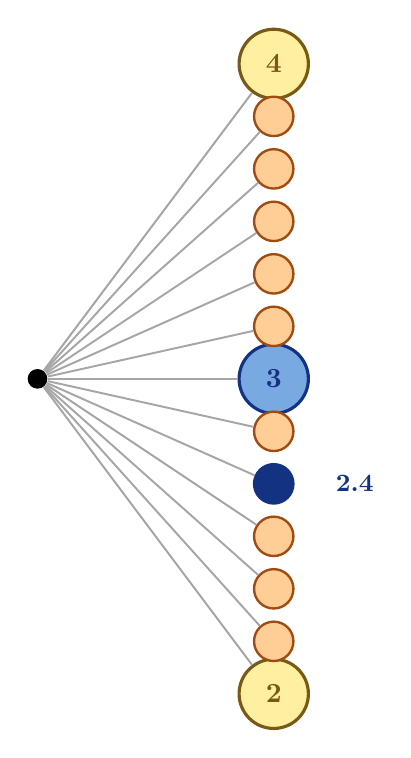
\begin{tikzpicture}[
  yscale=4,
  bigcircle/.style={circle, draw=darkyellow, fill=paleyellow, text=darkyellow,
                    minimum size=8.8mm, font=\bfseries, line width=0.4mm,
                    inner sep=0pt},
  bigoptcircle/.style={circle, draw=darkblue, fill=midblue, text=darkblue,
                       minimum size=8.8mm, font=\bfseries, line width=0.4mm,
                       inner sep=0pt},
  smallcircle/.style={circle, draw=darkorange, fill=paleorange,
                      minimum size=5mm, line width=0.3mm, inner sep=0pt},
  smalloptcircle/.style={circle, draw=darkblue, fill=darkblue,
                         minimum size=5mm, line width=0.3mm, inner sep=0pt},
  dotnode/.style={circle, fill=black, minimum size=2.5mm, inner sep=0pt}
]
  \node[dotnode] (p) at (-3, 3) {};

  \node[bigcircle]    (c2) at (0, 2) {2};
  \node[bigoptcircle] (c3) at (0, 3) {3};
  \node[bigcircle]    (c4) at (0, 4) {4};

  \foreach \k in {1,2,3,5} {
    \node[smallcircle] (s2\k) at (0, 2 + \k/6) {};
  }
  \node[smalloptcircle] (opt) at (0, 2 + 4/6) {};
  \node[anchor=west, text=darkblue, font=\small\bfseries]
        at ([xshift=4mm]opt.east) {2.4};

  \foreach \k in {1,...,5} {
    \node[smallcircle] (s3\k) at (0, 3 + \k/6) {};
  }

  \draw[gray!70, line width=0.25mm] (p) -- (c2);
  \draw[gray!70, line width=0.25mm] (p) -- (c3);
  \draw[gray!70, line width=0.25mm] (p) -- (c4);
  \foreach \k in {1,2,3,5} {
    \draw[gray!70, line width=0.25mm] (p) -- (s2\k);
  }
  \draw[gray!70, line width=0.25mm] (p) -- (opt);
  \foreach \k in {1,...,5} {
    \draw[gray!70, line width=0.25mm] (p) -- (s3\k);
  }
\end{tikzpicture}
\end{document}
